\section{Resultados e Discussão}

A Tabela \ref{tab:resultados_modelos} apresenta o desempenho quantitativo dos classificadores na partição de teste (20\% dos dados), ranqueados de forma decrescente pelo F1-Score. A escolha desta métrica justifica-se pelo forte desbalanceamento da base censitária, servindo como um avaliador mais robusto que a acurácia isolada (a qual atingiria facilmente 76\% através de um modelo ingênuo baseado apenas na classe majoritária).

\begin{table}[htbp]
\centering
\caption{Resultados dos modelos e seus melhores hiperparâmetros}
\label{tab:resultados_modelos}
\renewcommand{\arraystretch}{1.3} % Aumenta o espaçamento vertical entre as linhas
\resizebox{\textwidth}{!}{% % Garante que a tabela se ajuste perfeitamente à margem da página
\begin{tabular}{llllll}
\toprule
\textbf{Modelo} & \textbf{Parâmetro} & \textbf{Accuracy} & \textbf{Precision} & \textbf{Recall} & \textbf{F1} \\
\midrule
DecisionTree & criterion: 'gini' & 0.8563 ± 0.0048 & 0.7606 ± 0.0133 & 0.5840 ± 0.0238 & 0.6603 ± 0.0156 \\
             & max\_depth: 10 & & & & \\
             & min\_samples\_split: 2 & & & & \\
\midrule
LogisticRegression & C: 10 & 0.8503 ± 0.0060 & 0.7305 ± 0.0135 & 0.5940 ± 0.0206 & 0.6551 ± 0.0163 \\
\midrule
MLP & activation: 'relu' & 0.8403 ± 0.0057 & 0.6829 ± 0.0171 & 0.6241 ± 0.0449 & 0.6509 ± 0.0215 \\
    & alpha: 0.001 & & & & \\
    & hidden\_layer\_sizes: (64,) & & & & \\
\midrule
LinearSVM & C: 1 & 0.8503 ± 0.0059 & 0.7371 ± 0.0128 & 0.5826 ± 0.0208 & 0.6507 ± 0.0166 \\
\midrule
KNN & n\_neighbors: 11 & 0.8402 ± 0.0054 & 0.6899 ± 0.0140 & 0.6047 ± 0.0158 & 0.6444 ± 0.0126 \\
    & weights: 'uniform' & & & & \\
\midrule
GaussianNB & - & 0.5911 ± 0.0131 & 0.3626 ± 0.0076 & 0.9320 ± 0.0112 & 0.5220 ± 0.0085 \\
\bottomrule
\end{tabular}
}
\end{table}

A análise da tabela em conjunto com as matrizes de confusão revela claros padrões de generalização. A \textbf{Árvore de Decisão} obteve a melhor performance global (F1-Score 0.6603 e Precisão 0.7606). Ao registrar 1.433 verdadeiros positivos contra apenas 417 falsos positivos, o modelo comprovou sua aptidão para particionar o espaço de características e mapear interações complexas não lineares, conforme ilustrado na Figura \ref{fig:matriz_dt}.

\begin{figure}[htbp]
    \centering
    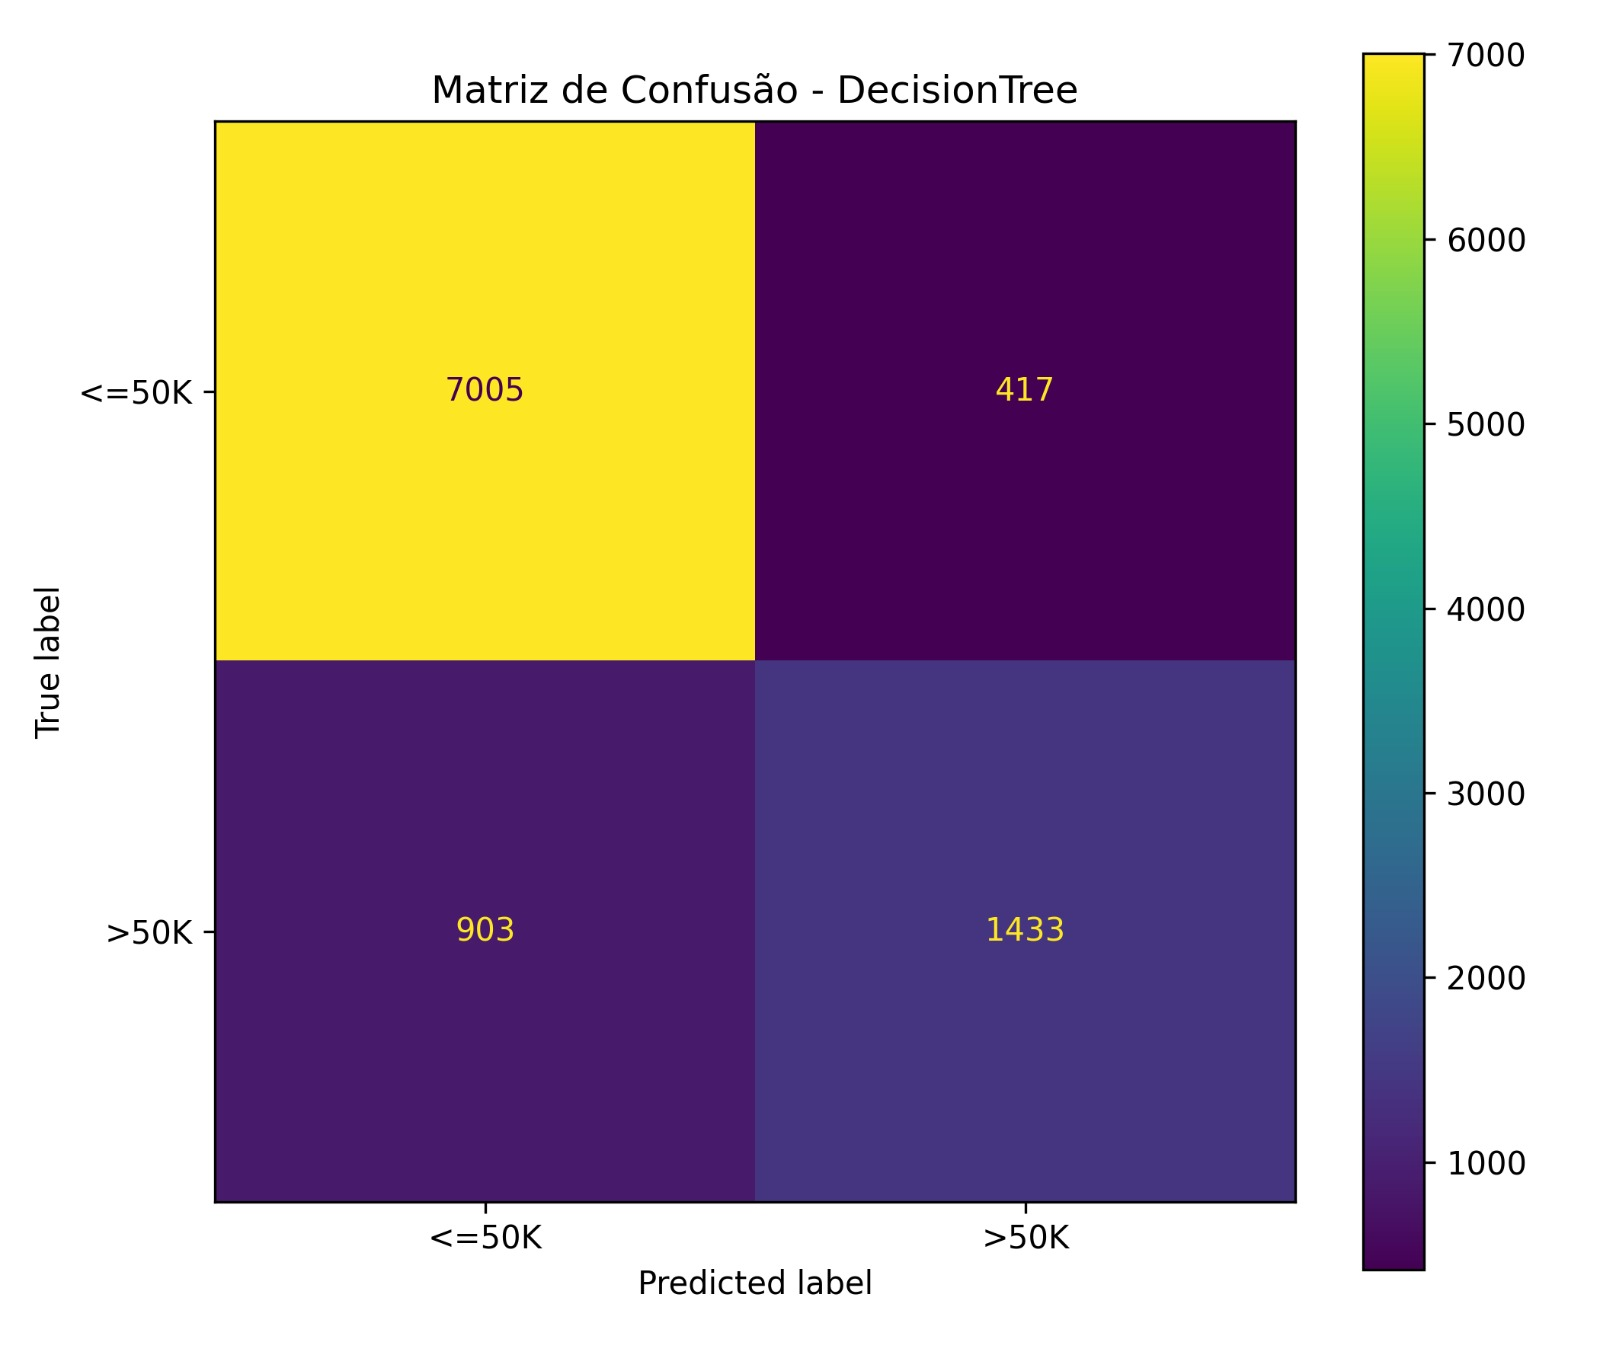
\includegraphics[width=0.5\textwidth]{Imagens/DecisionTree.jpeg}
    \caption{Matriz de Confusão para a Árvore de Decisão, evidenciando o melhor equilíbrio preditivo do experimento.}
    \label{fig:matriz_dt}
\end{figure}

Em um pelotão intermediário consistente, Regressão Logística, LinearSVM, MLP e KNN oscilaram entre 0.64 e 0.65 no F1-Score. A convergência destes estimadores foi diretamente garantida pela padronização \textit{Z-score} aplicada no pré-processamento. As matrizes dos modelos lineares (Regressão Logística e Linear SVM) e as abordagens não lineares de margem suave (MLP e KNN) exibiram comportamentos preditivos muito semelhantes, mantendo taxas de precisão competitivas (Figuras \ref{fig:matrizes_lineares} e \ref{fig:matrizes_nao_lineares}).

\begin{figure}[htbp]
    \centering
    \begin{minipage}{0.48\textwidth}
        \centering
        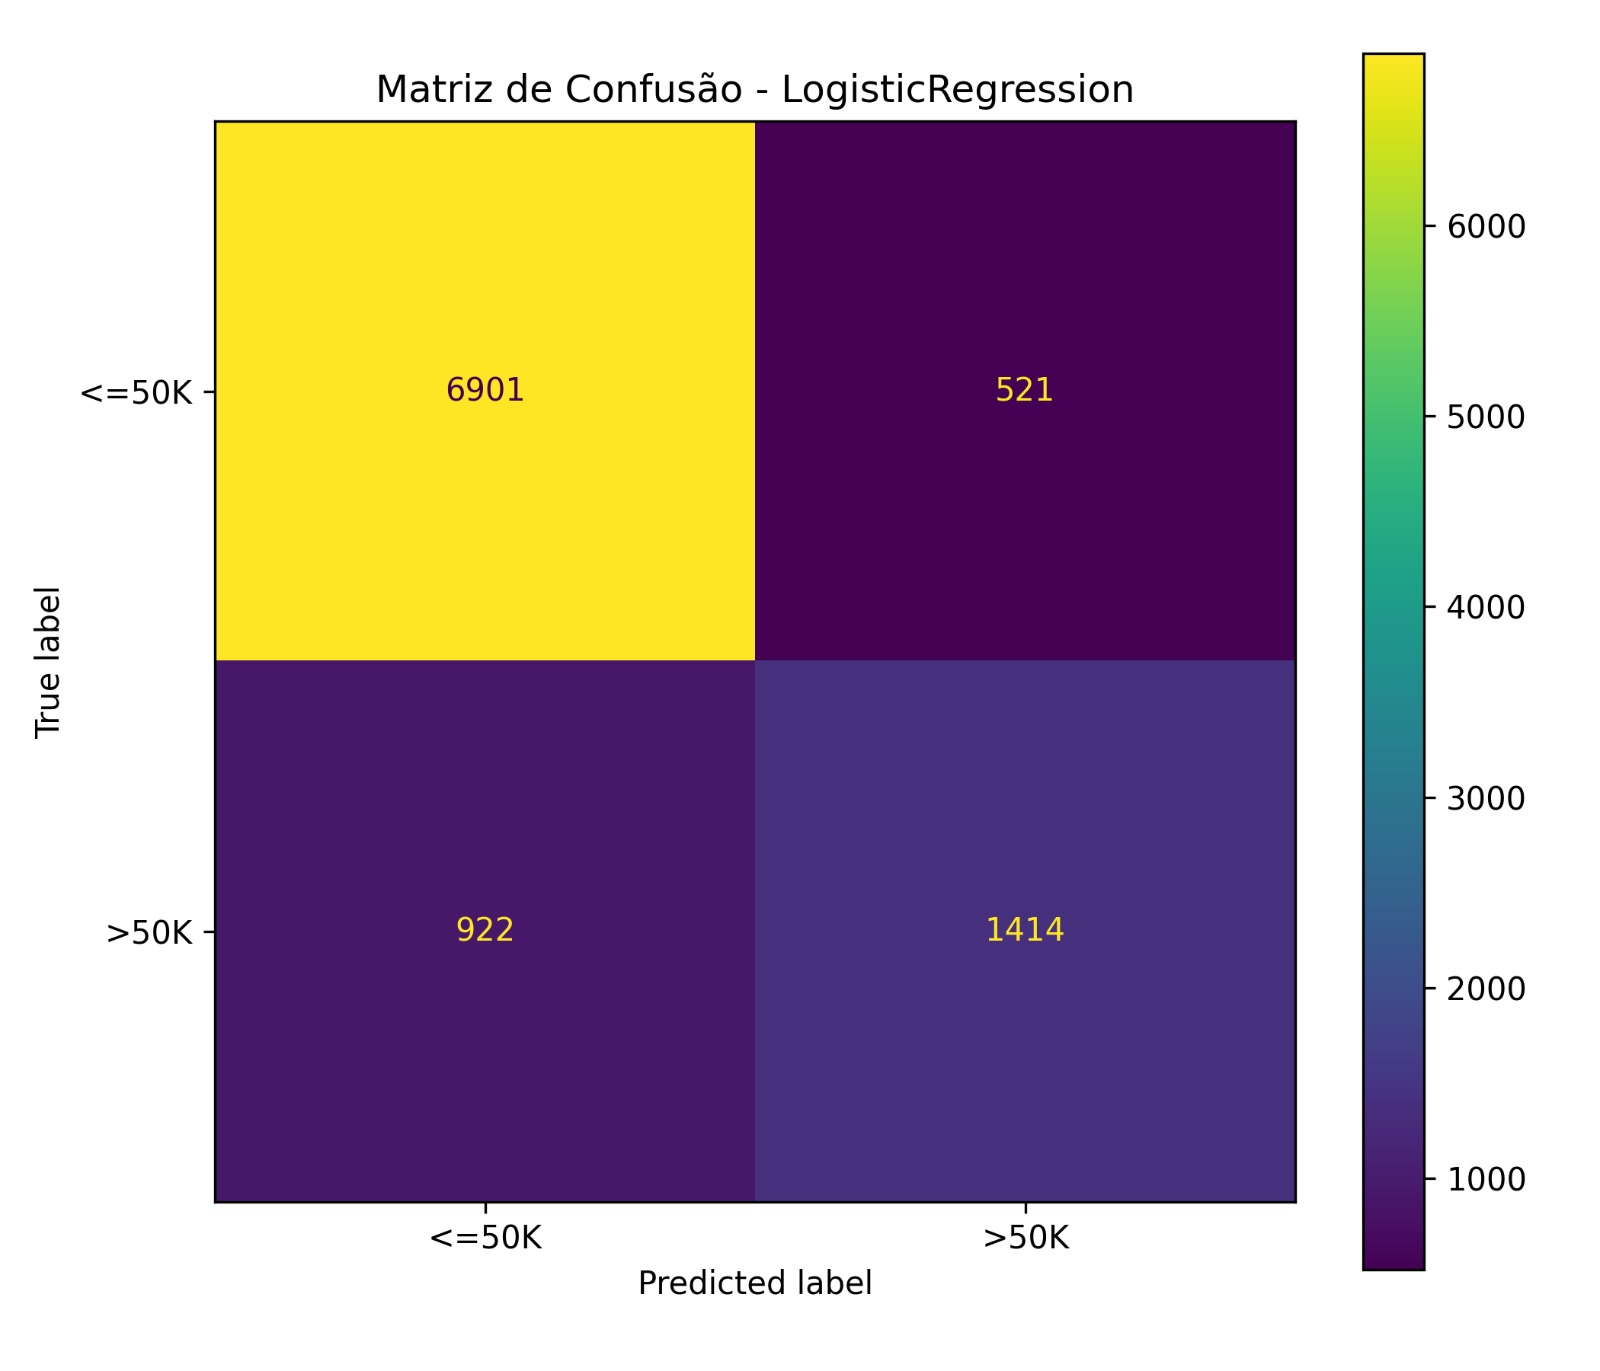
\includegraphics[width=\linewidth]{Imagens/LogisticRegression.jpeg}
        \caption*{Regressão Logística}
    \end{minipage}\hfill
    \begin{minipage}{0.48\textwidth}
        \centering
        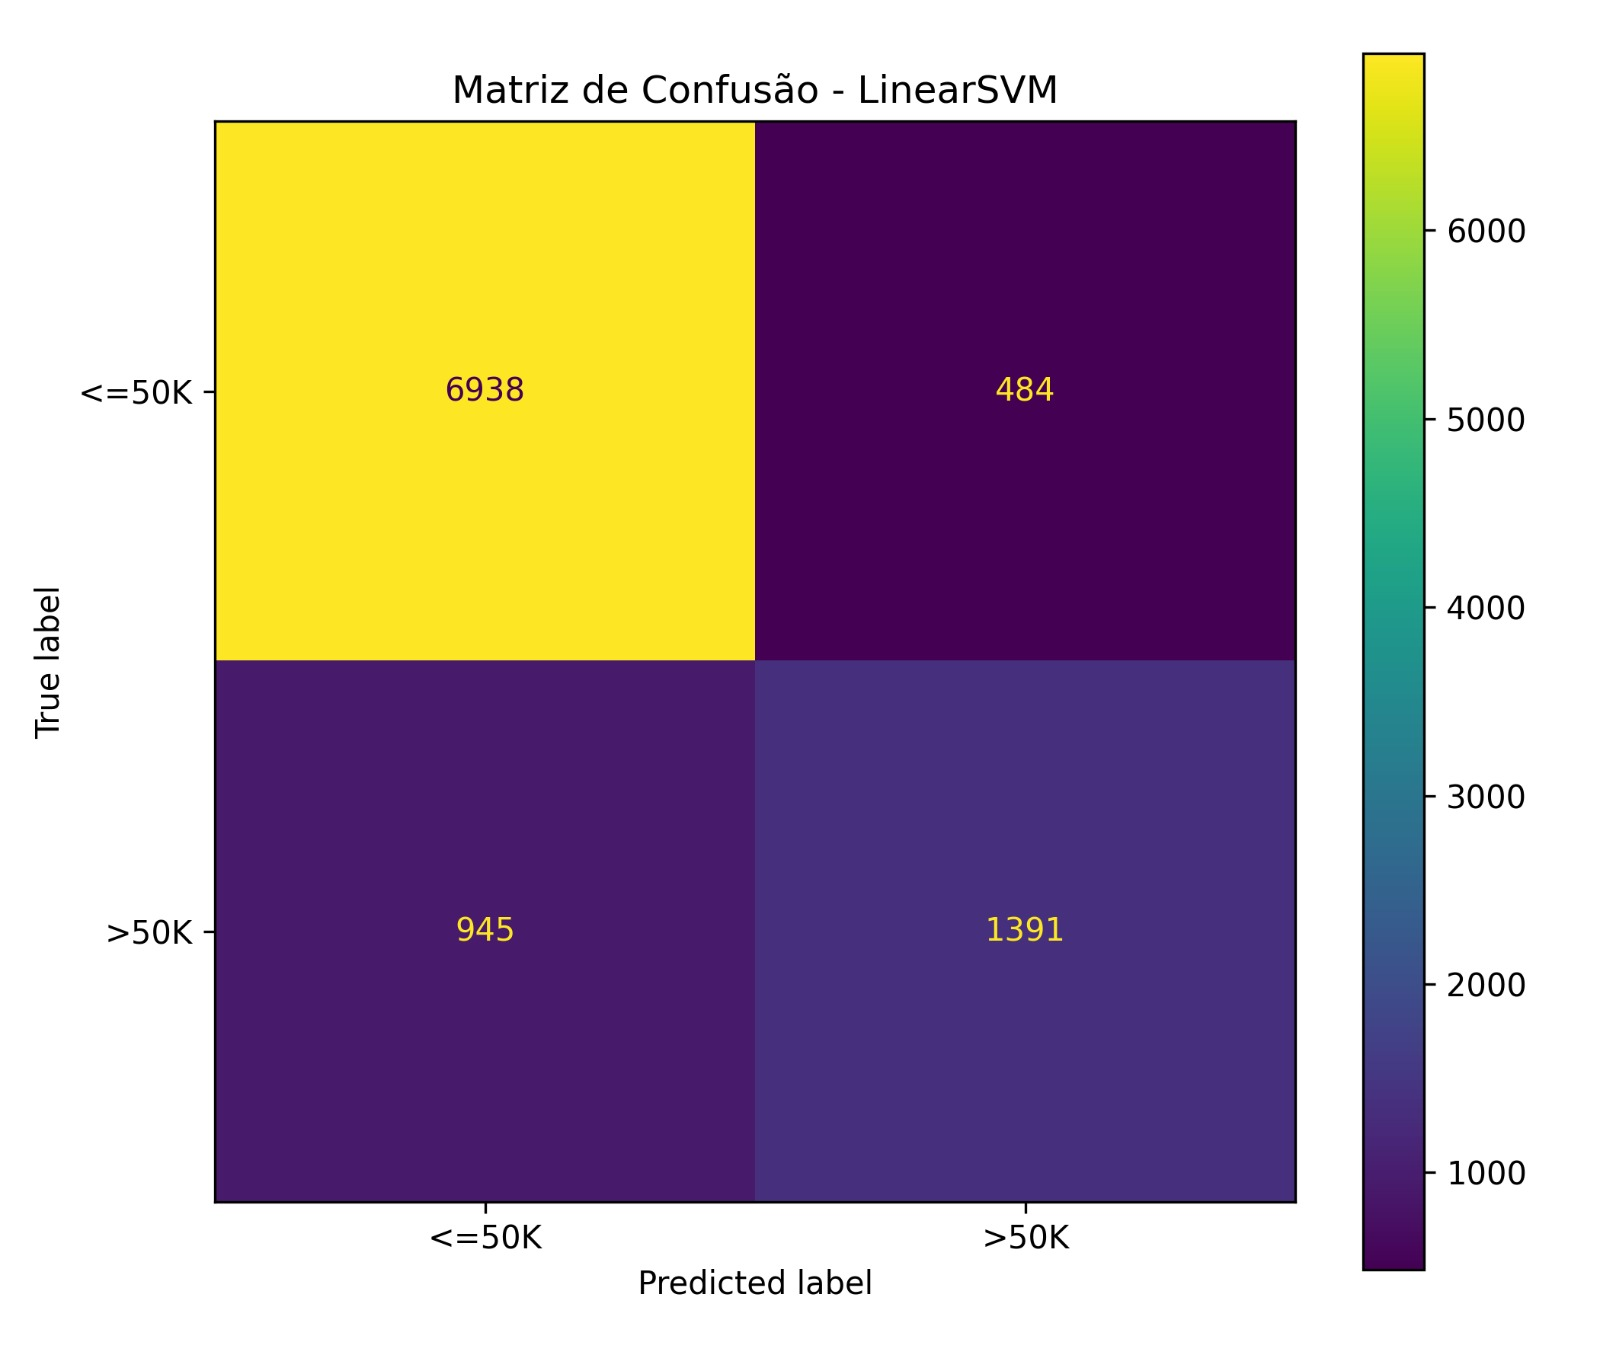
\includegraphics[width=\linewidth]{Imagens/LinearSVM.jpeg}
        \caption*{Linear SVM}
    \end{minipage}
    \caption{Matrizes de Confusão para os modelos lineares.}
    \label{fig:matrizes_lineares}
\end{figure}

\begin{figure}[htbp]
    \centering
    \begin{minipage}{0.48\textwidth}
        \centering
        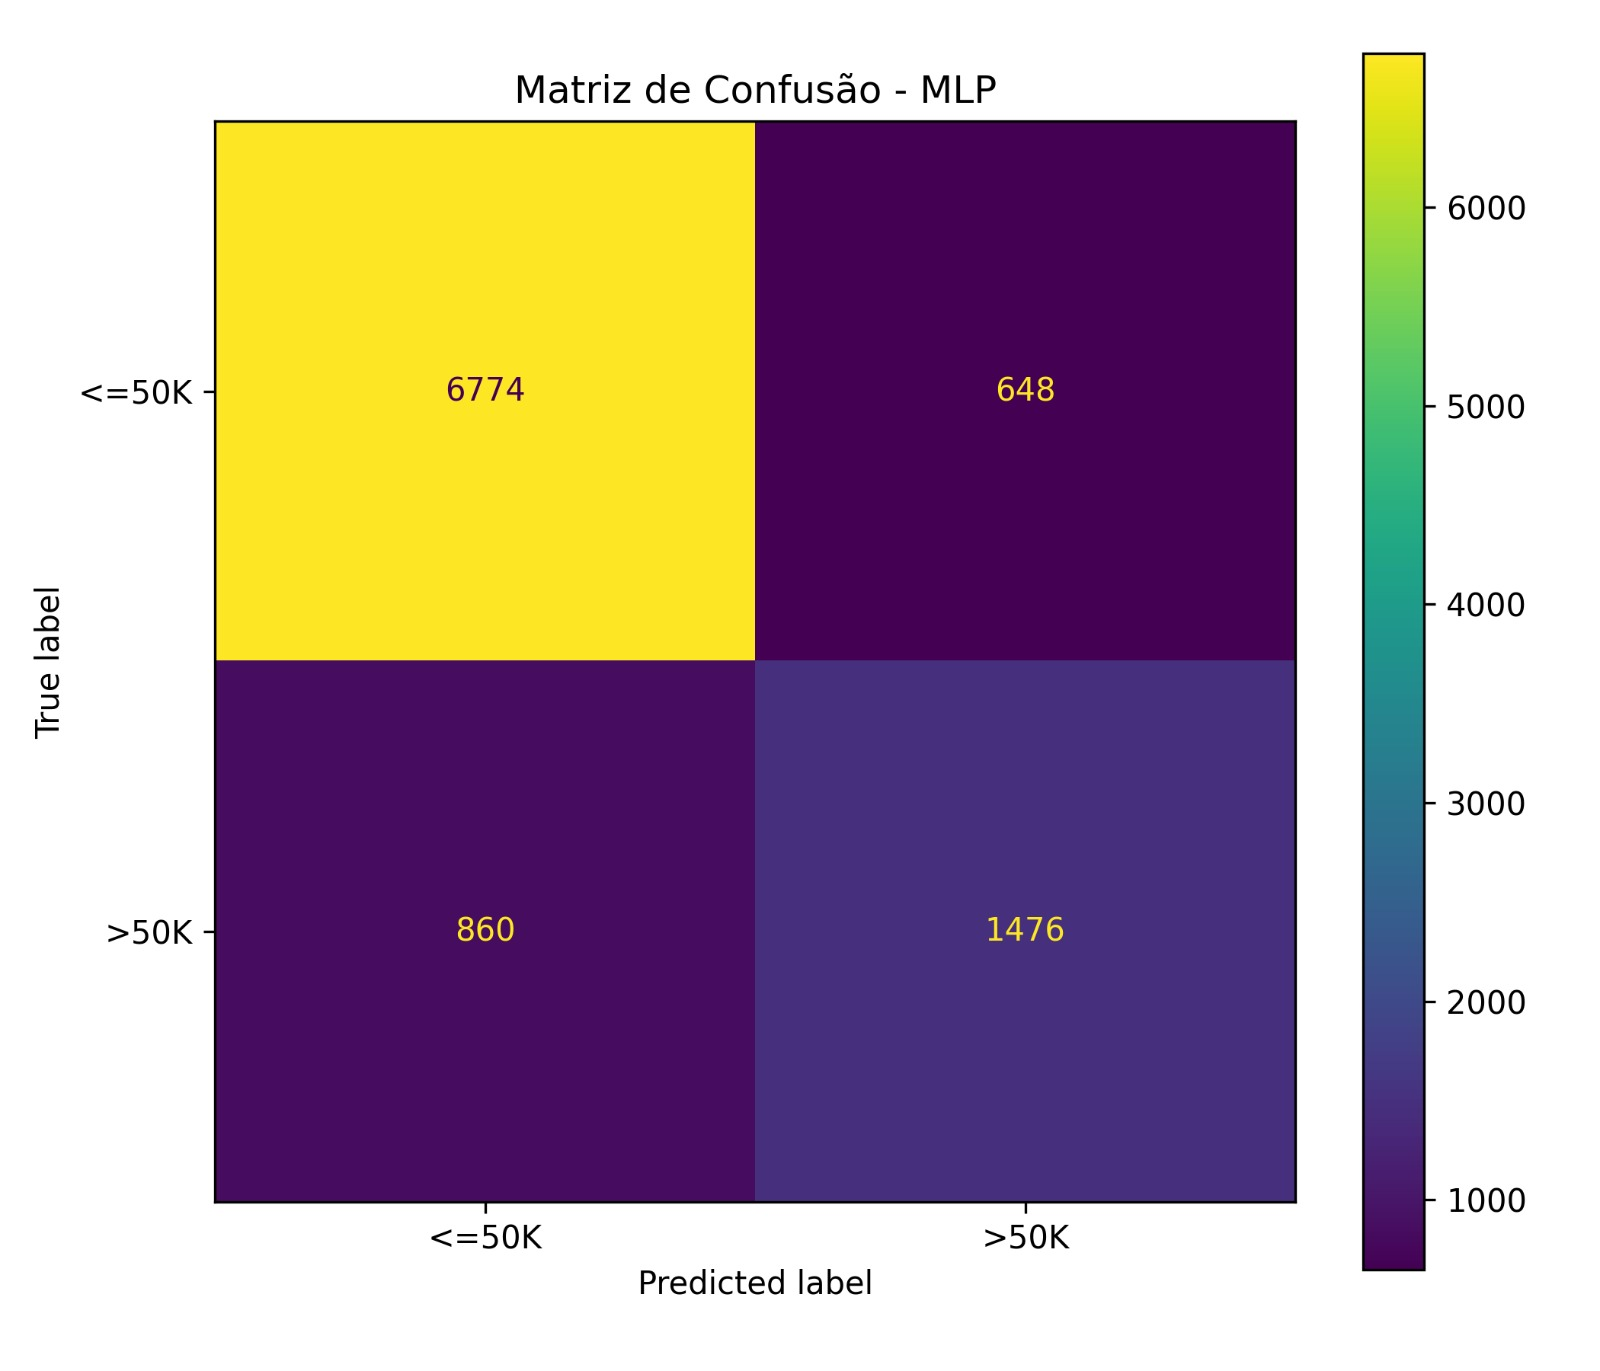
\includegraphics[width=\linewidth]{Imagens/MLP.jpeg}
        \caption*{Rede Neural (MLP)}
    \end{minipage}\hfill
    \begin{minipage}{0.48\textwidth}
        \centering
        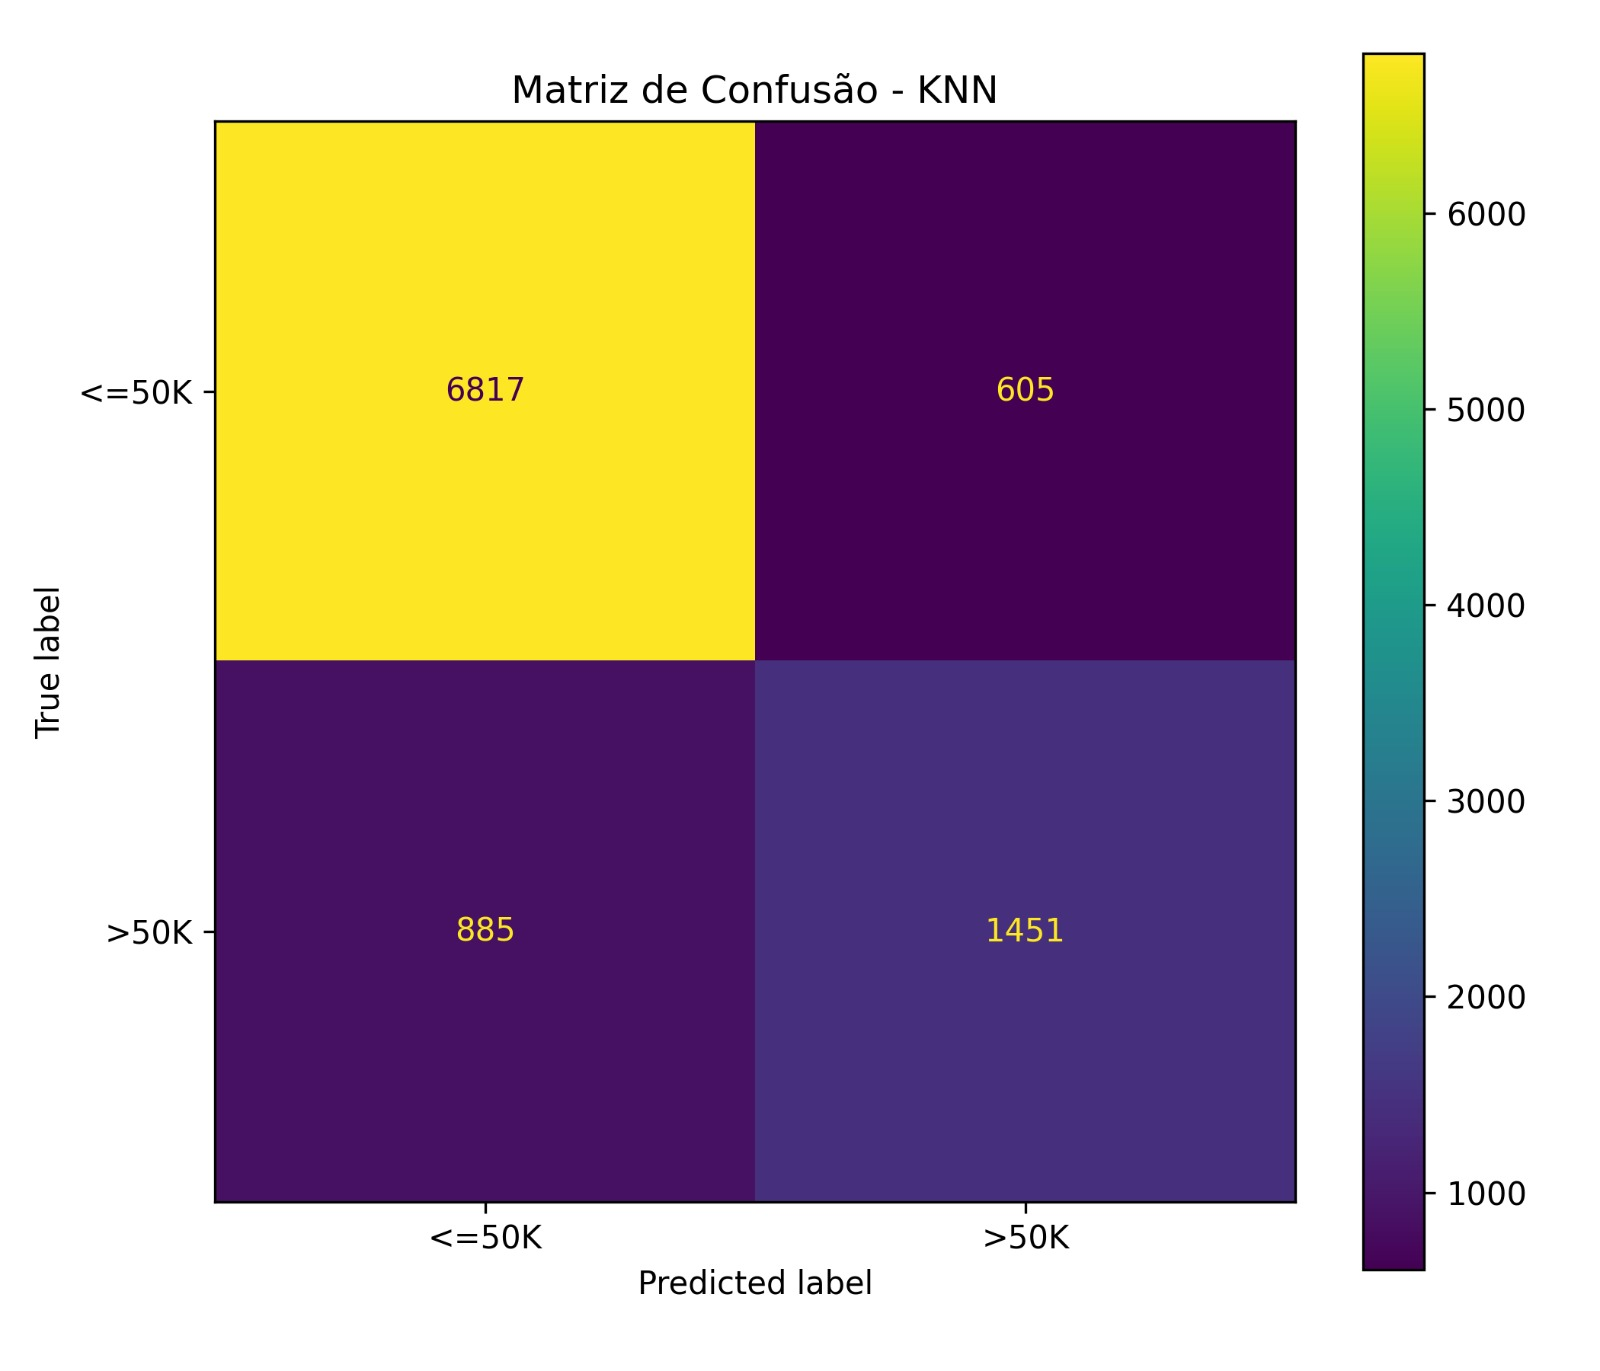
\includegraphics[width=\linewidth]{Imagens/KNN.jpeg}
        \caption*{KNN}
    \end{minipage}
    \caption{Matrizes de Confusão para o classificador MLP e KNN.}
    \label{fig:matrizes_nao_lineares}
\end{figure}

Já o \textbf{Naive Bayes Gaussiano} apresentou a pior métrica geral (F1-Score 0.5220) e a marca alarmante de 3.758 falsos positivos. A Figura \ref{fig:matriz_nb} reflete a forte penalização do modelo diante da violação da hipótese de independência condicional e da presença de atributos fortemente assimétricos, resultando na classificação incorreta massiva de indivíduos na classe minoritária.

\begin{figure}[H] % Forçando a imagem a ficar exatamente aqui
    \centering
    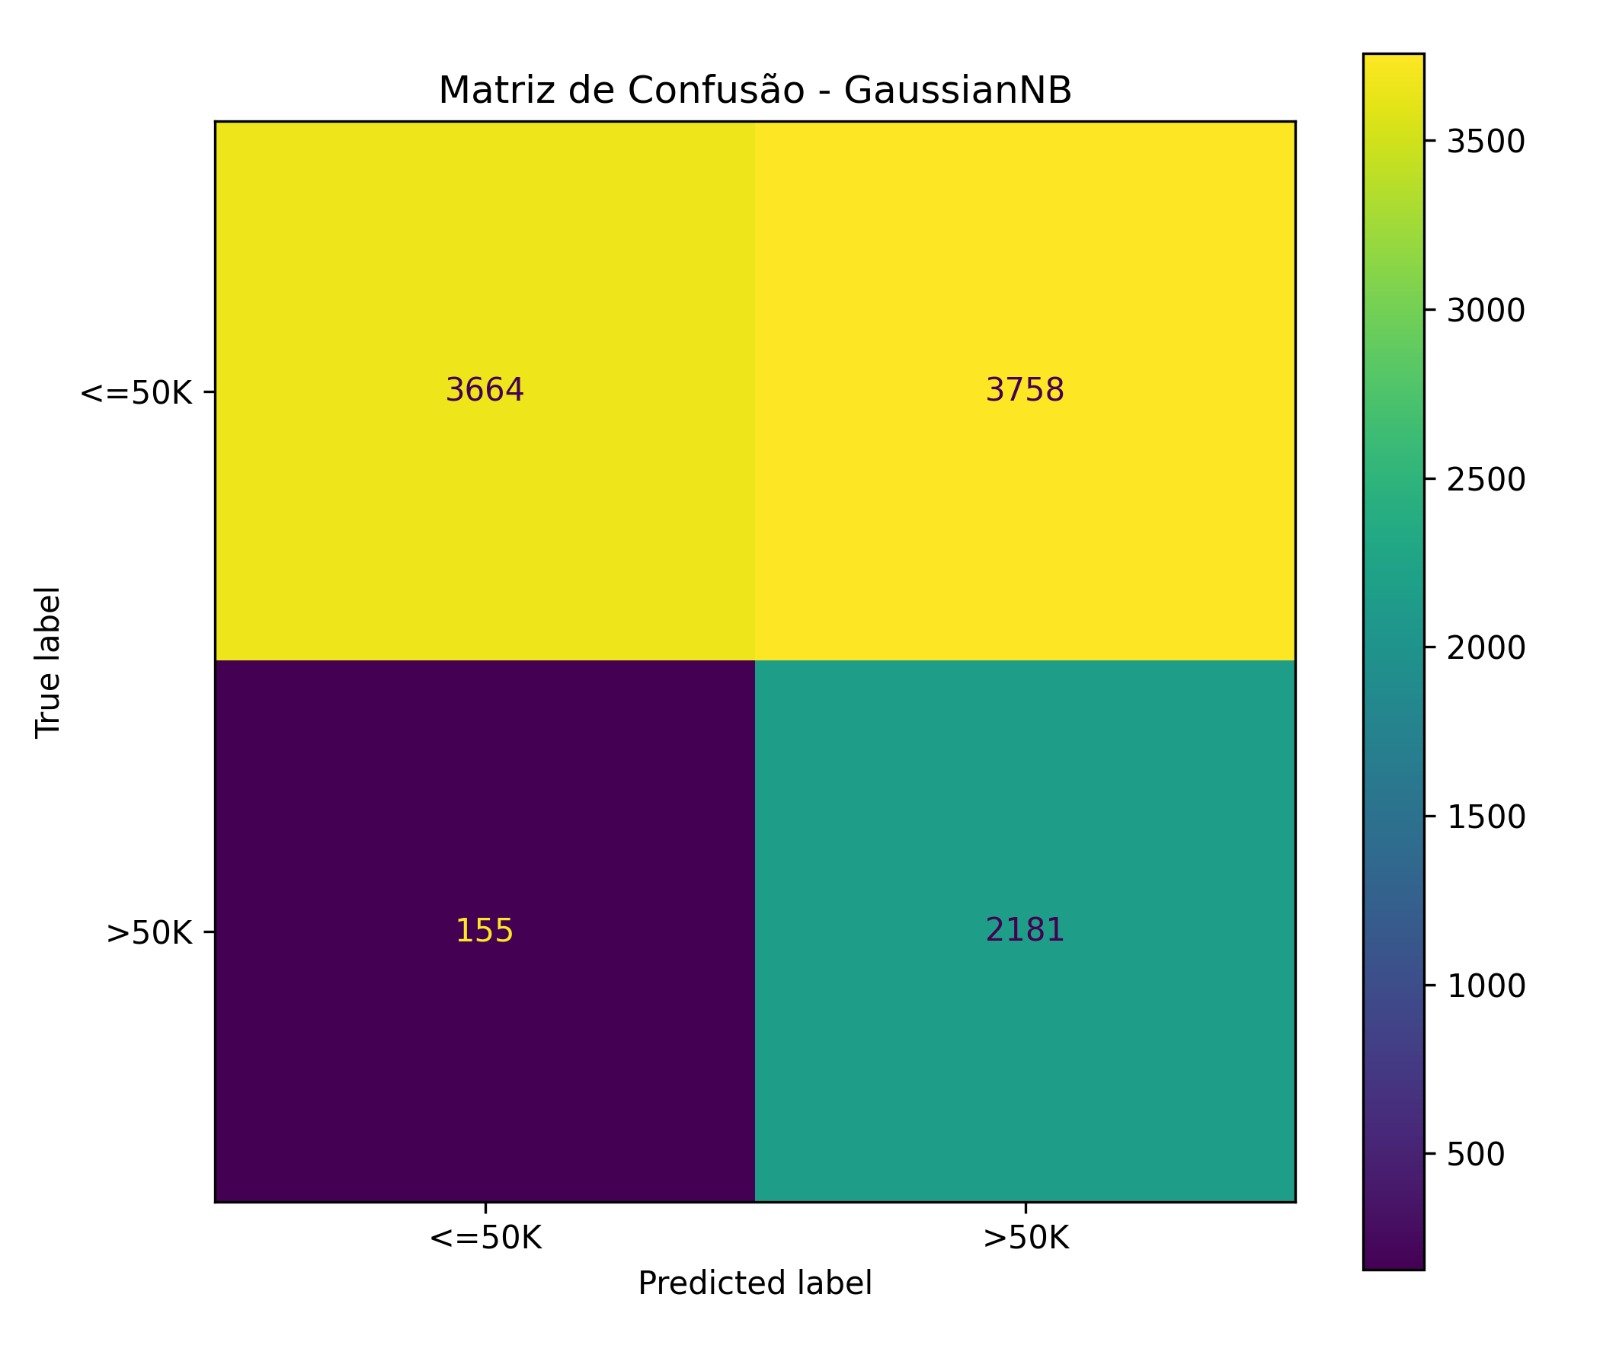
\includegraphics[width=0.4\textwidth]{Imagens/GaussianNB.jpeg} % Reduzido para 0.4 para caber no final da folha
    \caption{Matriz de Confusão para o Naive Bayes Gaussiano, destacando a discrepância e o alto volume de falsos positivos.}
    \label{fig:matriz_nb}
\end{figure}